\documentclass[12pt,a4paper]{ctexart}

\usepackage[a4paper,margin=2.5cm,headheight=25pt]{geometry}
\usepackage{graphicx}
\usepackage{booktabs}
\usepackage{array}
\usepackage{multirow}
\usepackage[table]{xcolor}
\usepackage{hyperref}
\usepackage{fancyhdr}
\usepackage{titlesec}
\usepackage{caption}
\usepackage{setspace}
\usepackage{enumitem}
\usepackage{lastpage}

\graphicspath{{./}}

\definecolor{TitleBlue}{HTML}{1F4E79}
\definecolor{LineBlue}{HTML}{D7E4F2}
\definecolor{SoftBlue}{HTML}{EEF4FB}
\definecolor{TextGray}{HTML}{5F6B7A}
\definecolor{TableHead}{HTML}{F3F7FB}

\hypersetup{
  colorlinks=true,
  linkcolor=TitleBlue,
  urlcolor=TitleBlue,
  citecolor=TitleBlue,
  pdftitle={关于我们 AI 辅导员产品形态与能力边界的建议},
  pdfauthor={OpenAI Codex},
  pdfsubject={AI 辅导员产品方案建议},
  pdfcreator={XeLaTeX}
}

\setstretch{1.28}
\setlength{\parskip}{0.35em}
\setlist[itemize]{leftmargin=2em,itemsep=0.2em,topsep=0.2em}
\setlist[enumerate]{leftmargin=2em,itemsep=0.2em,topsep=0.2em}
\captionsetup{font=small,labelfont=bf}

\titleformat{\section}{\Large\bfseries\color{TitleBlue}}{\thesection}{0.8em}{}
\titleformat{\subsection}{\large\bfseries\color{TitleBlue}}{\thesubsection}{0.8em}{}
\titlespacing*{\section}{0pt}{1.2em}{0.6em}
\titlespacing*{\subsection}{0pt}{0.8em}{0.4em}

\pagestyle{fancy}
\fancyhf{}
\fancyhead[L]{\small 关于我们 AI 辅导员产品形态与能力边界的建议}
\fancyhead[R]{\small 2026年6月}
\fancyfoot[L]{\small 阶段性建议稿}
\fancyfoot[R]{\small 第 \thepage\ 页 / 共 \pageref{LastPage} 页}
\renewcommand{\headrulewidth}{0.4pt}
\renewcommand{\footrulewidth}{0.4pt}
\renewcommand{\headrule}{\hbox to\headwidth{\color{LineBlue}\leaders\hrule height \headrulewidth\hfill}}
\renewcommand{\footrule}{\hbox to\headwidth{\color{LineBlue}\leaders\hrule height \footrulewidth\hfill}}

\newcommand{\summarybox}[1]{%
  \noindent
  \colorbox{SoftBlue}{%
    \parbox{\dimexpr\linewidth-2\fboxsep-8pt\relax}{\raggedright #1}
  }%
}

\begin{document}

\begin{titlepage}
  \thispagestyle{empty}
  \vspace*{2.8cm}

  {\centering
  {\fontsize{22pt}{30pt}\selectfont\bfseries\color{TitleBlue} 关于我们 AI 辅导员产品形态与能力边界的建议\par}
  \vspace{0.8cm}
  {\Large 围绕产品结构、能力组织与论坛边界的阶段性整理\par}
  \vspace{2cm}
  }

  \noindent\color{LineBlue}\rule{\linewidth}{1pt}
  \vspace{0.5cm}

  \noindent\textbf{文档类型}\hspace{1.6em} 产品建议报告\par
  \noindent\textbf{使用场景}\hspace{1.6em} \parbox[t]{0.72\linewidth}{AI 辅导员产品讨论、方案汇报、内部评审}\par
  \noindent\textbf{版本}\hspace{3.2em} V1.0\par
  \noindent\textbf{日期}\hspace{3.2em} 2026年6月\par

  \vfill

  \summarybox{\textbf{摘要说明：}本报告围绕 AI 辅导员的定位、首页结构、能力组织以及论坛能力的吸收边界展开，目标不是单纯优化视觉，而是帮助我们把产品从“聊天页思路”转向“学生服务工作台思路”，形成一套更适合校内正式场景、也更利于持续建设的产品框架。}

  \vfill

  {\small\color{TextGray}
  本材料为阶段性建议稿，重点用于产品方向讨论与界面结构说明。}
\end{titlepage}

\pagenumbering{Roman}

\section*{摘\quad 要}
我们认为，AI 辅导员如果要在校内场景真正发挥作用，其核心价值不应停留在“会回答问题”，而应进一步落到“能帮助学生把事情办下去”。从实际使用场景看，学生进入系统后最常见的诉求并不是自由聊天，而是查课表、看通知、找流程、交材料、联系部门等具有明确目标的任务。因此，产品结构应从“以聊天框为中心”转向“以任务、待办和可信信息为中心”，再由 AI 能力承担解释、引导和分发的工作。

在这个前提下，本报告对现有页面的主要问题进行了梳理，并提出了更适合校内正式场景的首页结构、能力分层与建设路径。同时，我们也对论坛能力是否值得吸收、以及以什么边界进入 AI 辅导员体系进行了分析。我们的基本结论是：论坛中与办事经验、案例沉淀和高频问题有关的部分具有明显价值，但不宜将完整论坛直接纳入，而更适合沉淀为经过治理的“经验问答层”。

\noindent\textbf{关键词：} AI 辅导员；学生服务工作台；能力编排；经验问答层；产品结构

\clearpage
\tableofcontents
\clearpage
\pagenumbering{arabic}

\section{我们的基本判断}
如果我们要把 AI 辅导员做成一个真正能长期使用的系统，那它的核心就不应该只是“会聊天”，而应该是“能帮学生把事情往下办”。学生进入这个页面，很多时候不是为了和 AI 对话本身，而是为了更快完成具体任务，比如查课表、看通知、找流程、交材料、联系部门。

所以从产品定位上看，我们更适合把它理解成一个学生服务工作台，而不是一个放大版聊天页。前者强调的是任务承接、能力组织和结果落点；后者强调的是对话本身。对于校内正式场景而言，真正的长期价值更可能来自前者。

\section{现有页面的主要问题}
现在这个版本最大的问题，不是视觉风格本身，而是结构重心有点偏。中间聊天区过重，占了页面最核心的位置，但没有承接最常见的校园任务；左侧历史会话、右侧快捷入口、常见问题，本质上又都在承担导航功能，信息较散，也存在重复。

另外，页面缺少足够明确的“和我有关”的内容。学生点进来之后，最先关心的通常是今天有没有课、最近有没有考试、有没有材料没交、最近有没有新通知，而不是一句欢迎语。AI 回答完之后，下一步动作也不够清楚，告诉用户流程是一回事，能不能顺着结果继续办完事，是另一回事。

对学校场景来说，页面中的可信度表达也很关键。来源、更新时间、适用对象、是否为官方口径，这些信息如果缺失，用户很容易把生成内容和正式结论混在一起。从这个角度看，现有版本更像是一个 AI 展示页，还不像一个真正能承接学生服务的 AI 辅导员。

\section{我们建议的产品定位}
我们更建议把 AI 辅导员定位成“学生服务工作台 + 对话式引导层”。这里的重点是，首页优先承接任务，对话能力负责做补充。AI 最有价值的地方，不是单纯生成一段回答，而是放在以下几个环节：

\begin{itemize}
  \item 帮学生判断问题属于哪类事务；
  \item 帮学生把分散信息整理成更好理解的结果；
  \item 帮学生进入正确的办理入口；
  \item 在复杂、模糊、跨系统的问题上继续追问和引导。
\end{itemize}

如果按这个方向做，AI 辅导员会更像一个可持续建设的校内系统，而不是一个阶段性的功能展示。它的核心不在于“回答得像不像人”，而在于“结果是否可信、流程是否可继续、任务是否能闭环”。

\section{首页重构方向}
这次重画首页的思路，就是把页面从“聊天中心”改成“任务中心”。首页更适合优先展示几类学生最关心的信息，比如“今日课表”“最近考试”“待交材料”“最新公告”。AI 输入框仍然保留，但不再独占页面中心，而是作为“描述复杂问题”或“补充说明”的入口。

在此基础上，首页应直接提供一组高频任务入口，例如“查课表”“查成绩”“办事流程”“提交材料”“联系部门”“校园公告”“宿舍电费”“常见问题”。右侧区域则不建议继续放静态介绍，而更适合放“我的待办”“办事进度”“可信来源”“最近咨询”这类真正有用的动态信息。

这样改的好处是，学生一进来就能明白两件事：第一，这个系统知道我现在最可能需要什么；第二，它不只是会回答问题，而是真的能帮我推进事情。

\begin{figure}[htbp]
  \centering
  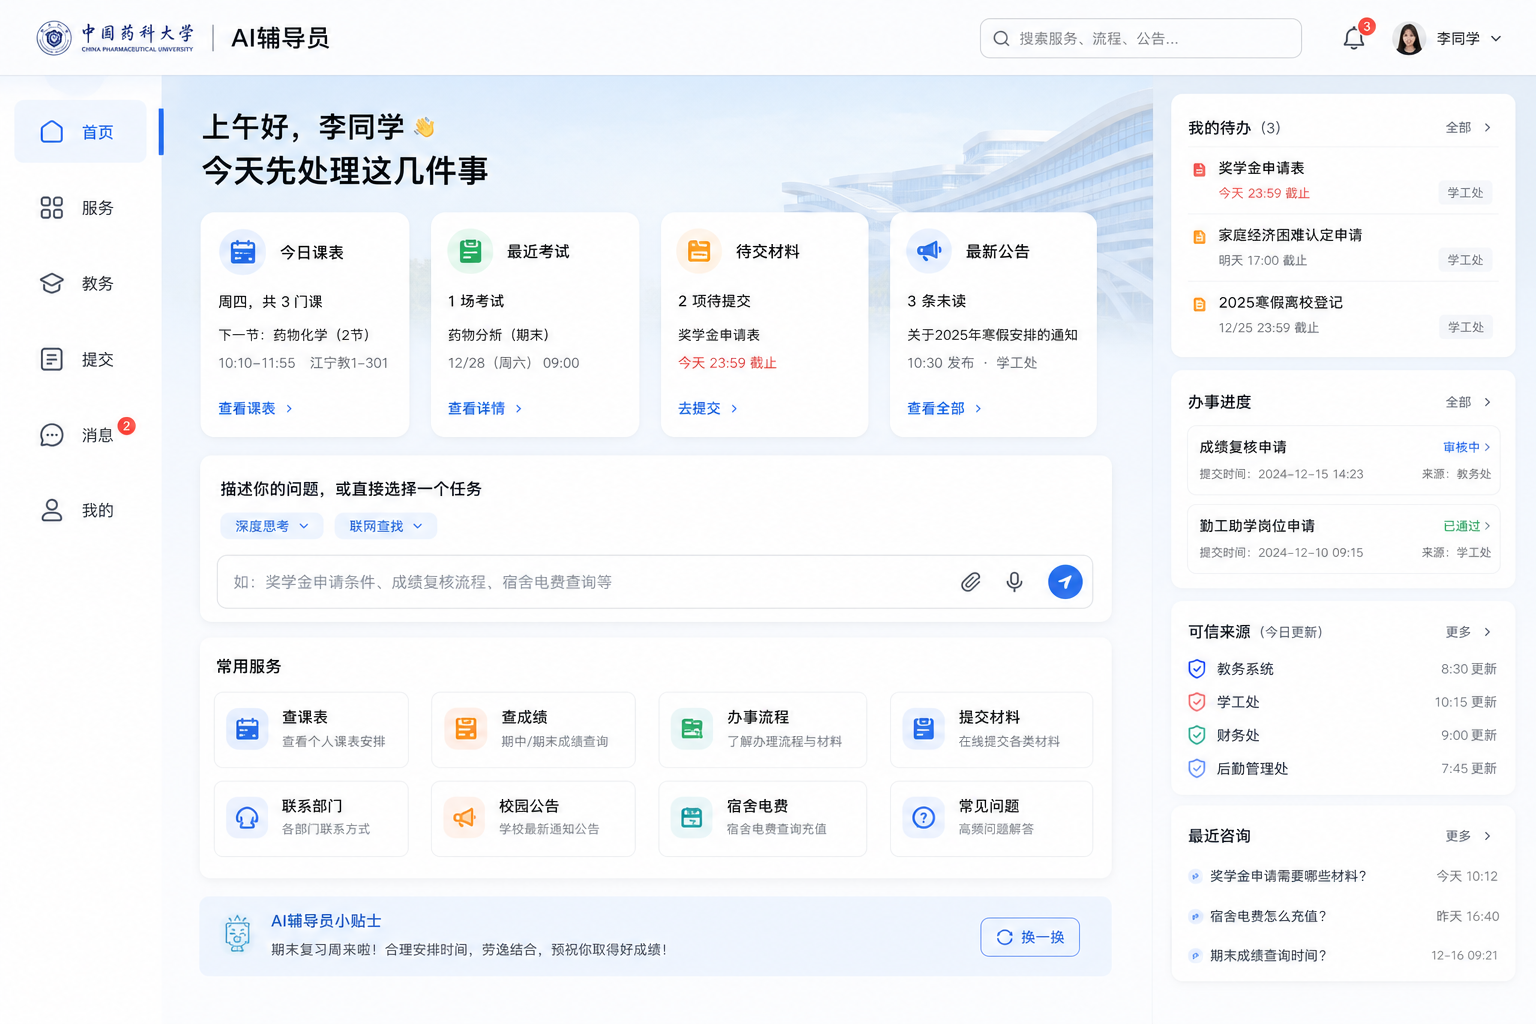
\includegraphics[width=0.94\textwidth]{01-homepage-workbench-concept.png}
  \caption{首页概念图：从“聊天中心”转向“任务中心”的工作台式首页}
\end{figure}

\section{我们真正值得吸收的部分}
如果我们要吸收现有项目中的一些能力，重点不应该放在照搬页面，而应该放在吸收背后的组织方式。更值得吸收的部分，不是一个具体界面，而是以下几类更底层的能力：

\begin{itemize}
  \item 把分散校园服务整理成统一入口的思路；
  \item 把高频任务拆成明确功能模块的思路；
  \item 教务、公告、问卷、文件收集、云盘这类轻能力的组织方式；
  \item 哪些内容可公开、哪些必须登录、哪些只能本人查看的权限边界；
  \item AI 回答之后，如何把用户送到真正的办理入口，而不是停留在一段文字里。
\end{itemize}

简单说，真正有价值的不是一个站点皮肤，而是“服务整合能力”和“任务落地能力”。如果这一层吸收得好，后续无论界面细节如何调整，整体产品方向都会更稳。

\subsection{能力结构建议}
从系统建设角度看，我们更适合把 AI 辅导员拆成“展示层、AI 编排层、能力与数据层”三部分。展示层负责承接首页工作台、任务卡片、对话入口和结果卡片；AI 编排层负责意图识别、问题分类、工具调用、结果整理和下一步引导；能力与数据层则承接教务数据、校园公告、办事流程、材料提交、问卷收集、联系方式以及经验问答层等实际能力。

这种分层方式的好处在于，页面展示不会和底层接口强耦合，AI 能力也不会被迫变成一个“大而全的聊天接口”。系统后续扩展时，既可以新增能力，也可以单独优化结果组织方式，整体演进空间会更大。

\begin{figure}[htbp]
  \centering
  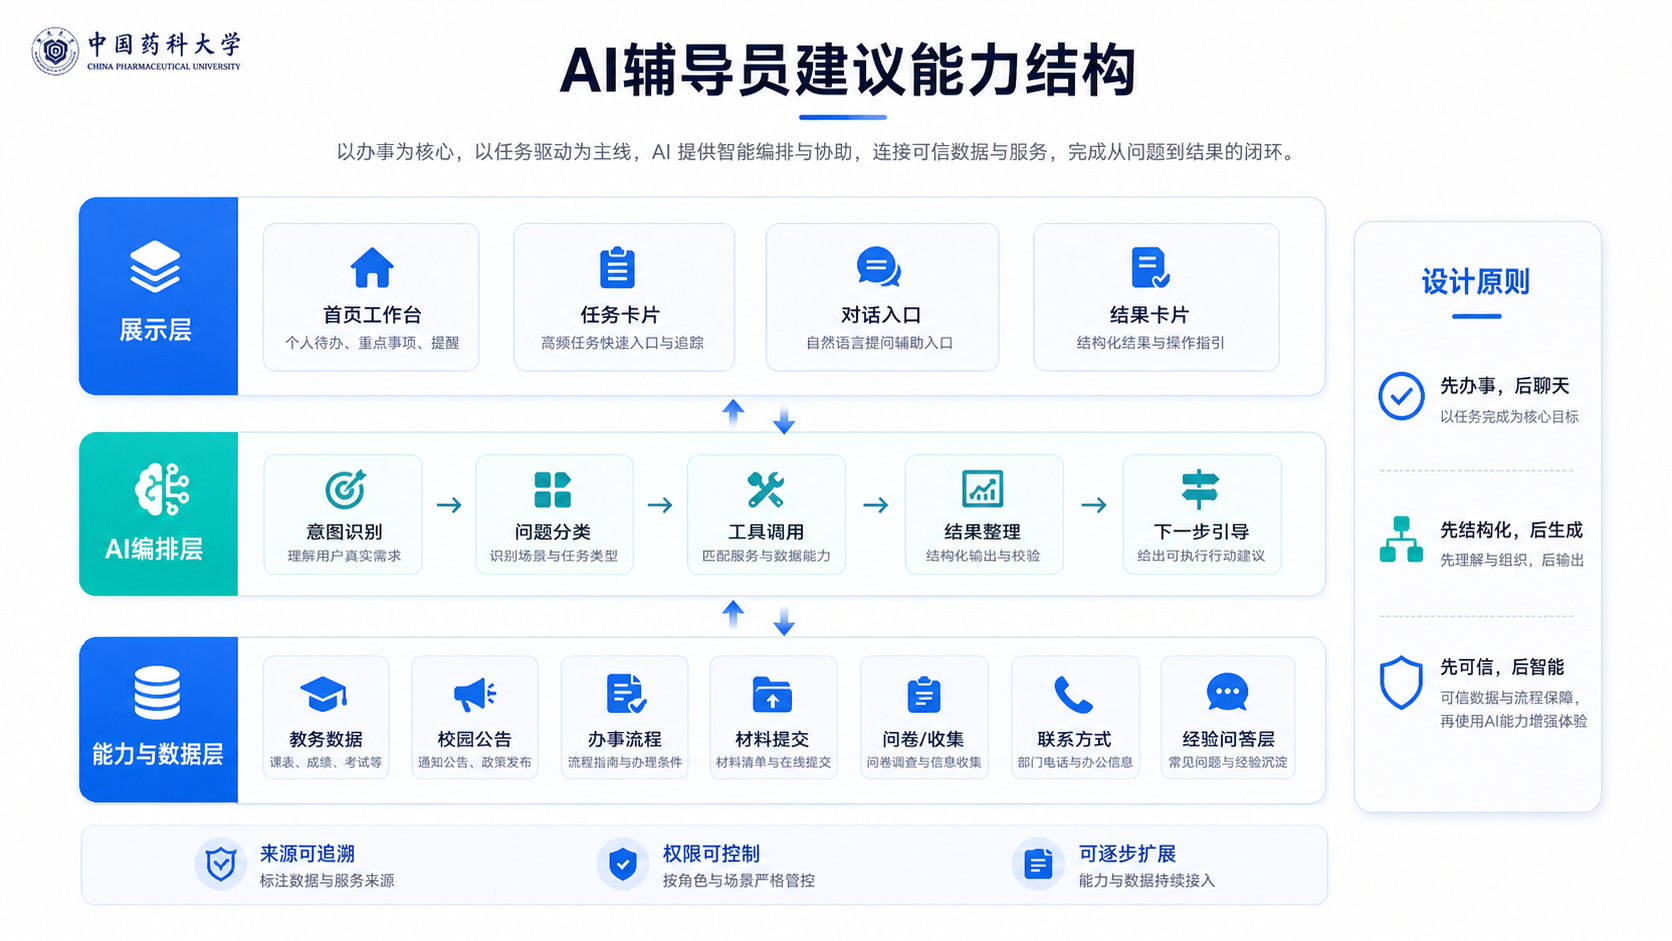
\includegraphics[width=0.92\textwidth]{02-capability-architecture.png}
  \caption{能力结构图：展示层、AI 编排层与能力数据层的分层关系}
\end{figure}

\section{关于论坛能力，能不能吸收}
我们认为，论坛能力可以吸收一部分，但不建议把完整论坛直接并进 AI 辅导员。论坛类内容的价值很明显，它能补足纯官方知识库覆盖不到的实际经验，比如某个流程里容易卡住的地方、材料提交时常见的问题、学生真实会怎么提问。它也能持续沉淀新的问题场景，让系统不是只会回答预设 FAQ，而是能不断接近真实使用。

但问题也同样明显。一旦进入官方系统，论坛就不再只是社区功能，而会带上很强的治理属性。开放灌水、强匿名吐槽、未经整理的自由讨论、二手交易这类内容，如果直接并进来，风险会很高，也会把产品重心带偏。

因此，更合适的方式不是“把完整论坛搬进来”，而是把其中最有价值、最可治理的部分提炼出来，做成一个经验问答层或案例知识层。这一层更适合承接：

\begin{itemize}
  \item 已解决问题；
  \item 办事经验整理；
  \item 高频咨询归档；
  \item 常见踩坑提醒；
  \item 经审核后的学生经验补充。
\end{itemize}

这里最关键的一点，是要把“官方信息”和“学生经验”明确分层。官方信息优先，学生经验单独标注，来源要清晰，AI 如果引用经验内容，也要能追溯到具体出处。这样论坛能力才能真正成为补充，而不是干扰。

\begin{figure}[htbp]
  \centering
  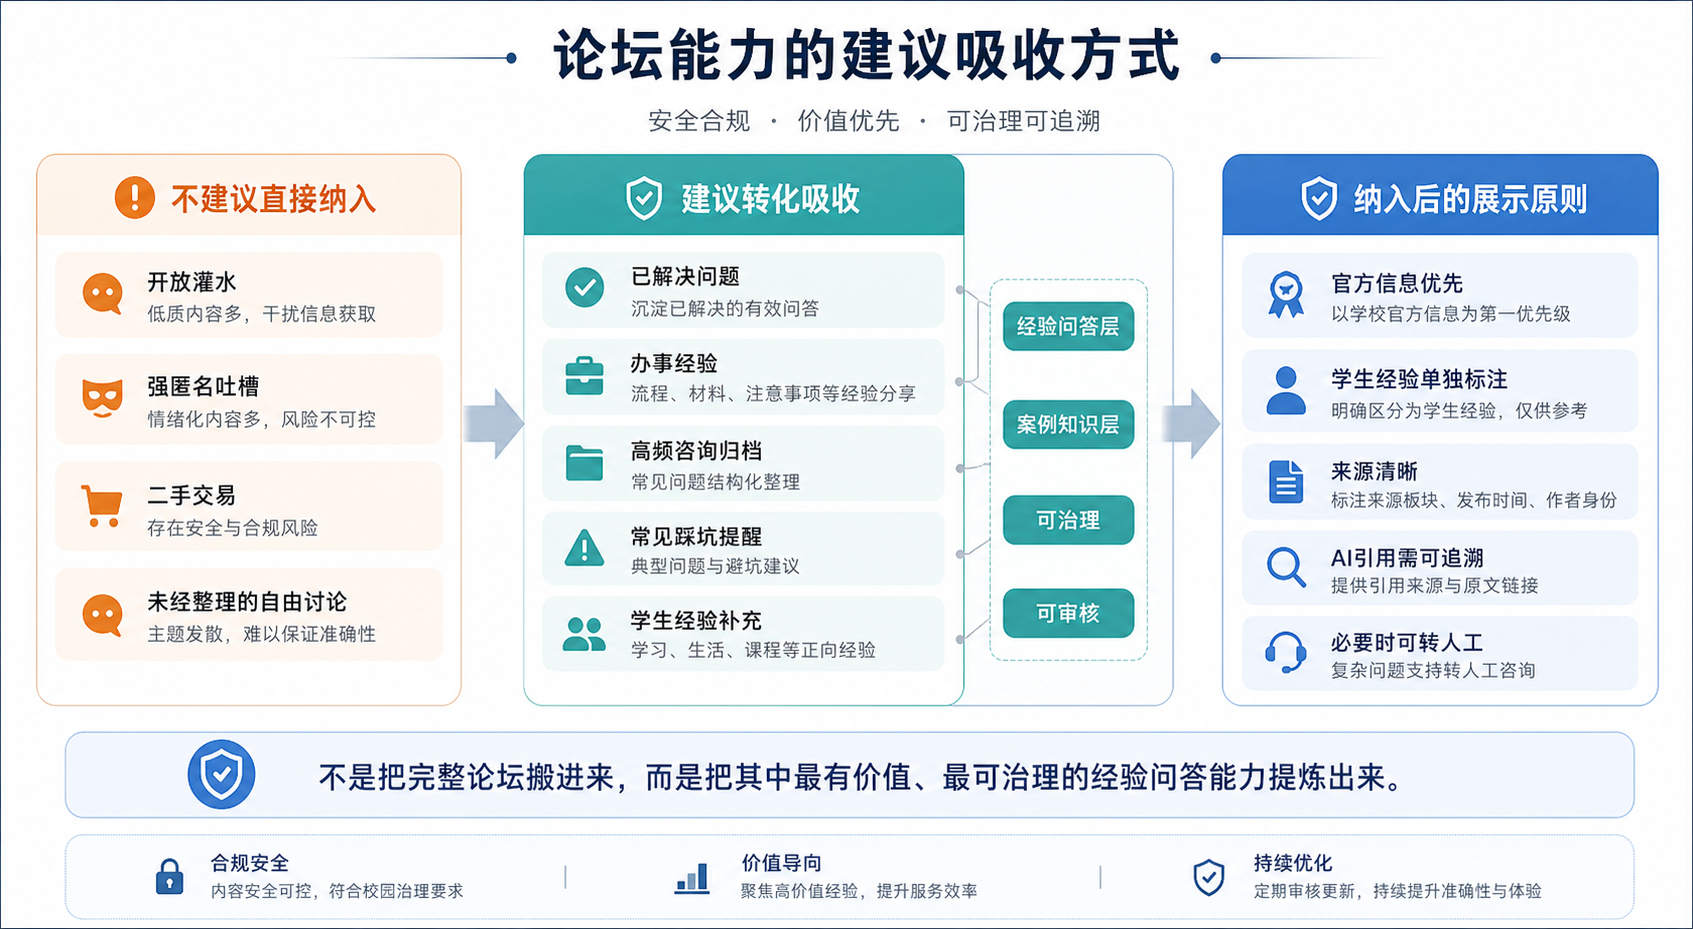
\includegraphics[width=0.92\textwidth]{03-forum-boundary.png}
  \caption{论坛边界图：保留经验价值，但避免把完整社区直接带入官方场景}
\end{figure}

\section{我们的推进建议}
从落地顺序上看，我们建议先把基础层做稳，再逐步扩展。一个更稳妥的推进路径可以分为四个阶段：

\begin{enumerate}
  \item 第一阶段先做好只读型能力，比如公告问答、流程解释、课表查询、成绩查询、考试信息、联系方式查询；
  \item 第二阶段再接入任务型能力，比如材料提交、问卷填写、办事进度查看、常见业务入口跳转；
  \item 第三阶段逐步加入个性化看板，根据学生身份、时间节点和任务状态展示待办事项；
  \item 第四阶段再考虑接入经过治理的经验问答层，把论坛里真正有价值的部分沉淀进来。
\end{enumerate}

这样的推进方式，一方面风险更可控，另一方面也更符合校内系统建设的节奏。先把可信信息和高频能力打稳，再逐步向复杂交互和经验层扩展，整体结构会更容易立住。

\subsection{建议原则归纳}
\begin{table}[htbp]
  \centering
  \caption{AI 辅导员建设的三条核心原则}
  \renewcommand{\arraystretch}{1.35}
  \begin{tabular}{ll}
    \toprule
    \rowcolor{TableHead}
    原则 & 说明 \\
    \midrule
    先办事，后聊天 & \parbox[t]{10.4cm}{优先承接任务、流程和入口，再让对话能力补足模糊场景，而不是让聊天成为唯一入口。} \\
    先结构化，后生成 & \parbox[t]{10.4cm}{能做成卡片、表单、步骤、来源说明的内容，优先结构化呈现，减少对纯文本生成的依赖。} \\
    先可信，后智能 & \parbox[t]{10.4cm}{在学校场景中，来源、更新时间、适用对象和权限边界始终优先于“回答听起来聪明”。} \\
    \bottomrule
  \end{tabular}
\end{table}

\section{结论}
我们的核心问题，其实不是首页要不要更好看，而是整个 AI 辅导员到底按什么思路来做。如果继续沿着“聊天页”去堆功能，它很容易停留在“会回答，但不太会办事”的状态。更合适的方向，是把它做成一个以任务、待办和可信信息为中心的学生服务工作台，再让 AI 去承担解释、引导和分发的工作。

如果我们要吸收现有项目中的价值，重点应该放在服务整合、能力编排、权限边界和任务落地这些方面。至于论坛能力，可以吸收，但必须收边界、做治理，更适合沉淀成经验问答层，而不是直接引入一个完整社区。

总的来说，这个产品真正值得追求的，不是“像一个更聪明的聊天框”，而是“像一个更懂校园场景、更能帮助学生把事情办下去的系统”。

\appendix
\section{配图使用建议}
三张配图分别对应不同的汇报重点：
\begin{itemize}
  \item 首页概念图适合放在汇报前半部分，用来直观说明“为什么首页应该从聊天中心转成任务中心”；
  \item 能力结构图适合放在中段，用来说明 AI 辅导员不是单一模型页面，而是展示层、AI 编排层和能力数据层共同组成的系统；
  \item 论坛边界图适合放在后半部分，用来说明论坛能力可以吸收，但必须经过治理和重构，不能直接以完整社区形态并入。
\end{itemize}

\end{document}
